\graphicspath{{./figures/}}
\chapter{Implementation}
This chapter focuses on the overall project's implementation.
It mainly covers the four parts hardware assembly, long jump analysis,
drone control and their consolidation into one \ac{GUI}.

\section{Hardware}\label{sec:4_hardware}
In order to capture high-quality video recordings that cover a complete long 
jump, from the first step all the way to the landing, a drone is used to fly
next to the athlete throughout the whole process.
Thus, a drone in form of a quadcopter is built from scratch.
Its control will be integrated seamlessly in the projects' \ac{GUI}.\\
This section introduces the hardware components that are used for building 
this drone as well as its flight control unit.\\
A short outline of the hardware is given in.
The assembly is shown in, while ... focuses on the PixHawk flight 
controller and its setup.

\subsection{Hardware selection}\label{subsec:4_hardware_selection}
Currently, commercial drone hardware on the market is mainly separable into 
the two large areas of fully remote controlled \ac{FPV} hardware and hardware 
for (autonomous) drones that can usually carry more load, e.g.~heavy cameras.
Even though the quadcopter in this project needs to be remotely 
controllable from a ground station pc, it is still more likely to be located 
in the latter one.\\
Generally the hardware was chosen based on the following criteria:
\begin{itemize}
    \item price
    \item compatibility
    \item size
\end{itemize}

\subsection*{Flight Hardware}\label{subsec:4_filght_hardware}
The main hardware that a quadcopter needs to fly will, in the following, be
referred to as \textit{flight hardware}.
This includes frame, motors, rotors, \acp{ESC} and a \ac{PDB}.\\
The main platform on which all drone hardware is mounted, is referred to as
a quadcopter's frame.
As this project's drone does not need to carry any heavy load, such as high 
precision camera systems or other sensors, a rather compact frame would 
theoretically be sufficient.
However, compact frames tend to be less stable compared to larger frame sizes 
which could lead to a lower video recording quality and thus require more 
complex post-processing software.
Moreover, the assembly process on larger frames is more convenient and 
replacing parts is easier.
Additionally, compact frames are most commonly used in areas that demand quick
reaction times for high speed flight maneuvers, e.g.~in drone racing.
This however is not needed in this project's context.\\
Taken the mentioned considerations into account the mid-sizes \textit{Holybro 
S500 V2} frame kit is chosen.
Besides the frame, the kit also includes a landing gear and rotors.
Moreover, the main platform includes a \ac{PDB} to split the battery's power 
equally to all four motors.\\
An overview of all included parts is given in \autoref{fig:4_frame_kit}.
\begin{figure}[!h]
    \centering
    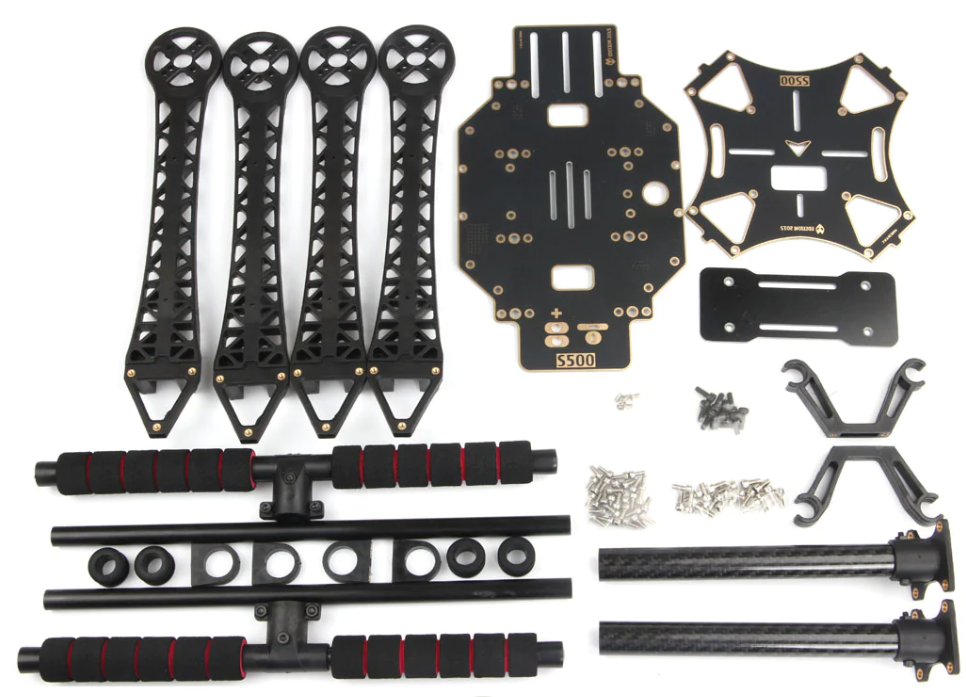
\includegraphics[scale=0.6]{frame-kit.png}
    \caption[Frame kit]{Holybro S500 V2 frame kit}
    \label{fig:4_frame_kit}
\end{figure}
\FloatBarrier
\noindent Besides the frame, motors and compatible \acp{ESC} are crucial 
flight hardware components.
Each motor requires an own \ac{ESC} that translates signals from a flight 
control unit to a voltage and thereby control the motors' rotation speed.
To guarantee compatibility, both components were chosen from Holybro as well
and can be seen in \autoref{fig:motors_and_esc}.
\begin{figure}[!h]
    \begin{subfigure}[b]{0.48\textwidth}
        \includegraphics*[scale=0.15]{motor.jpg}
        \caption{920KV Motor}
        \label{subfig:motor_picture}
    \end{subfigure}
    \hfill
    \begin{subfigure}[b]{0.5\textwidth}
        \includegraphics*[scale=0.15]{esc.jpg}
        \caption{\acl*{ESC}}
        \label{subfig:esc_picture}
    \end{subfigure}
    \caption[Motor and \acs*{ESC}]{Motor (a) and \acs*{ESC} (b)}
    \label{fig:motors_and_esc}
\end{figure}
\FloatBarrier
The drones' motors performance capabilities are defined by the number of 
\ac{RPM} they can perform per 1V input.
As can be seen in \autoref{subfig:motor_picture}, this link between 
rotation speed and input voltage is expressed in the arbitrary unit \textit{KV}.
The chosen motors are capable of rotate with a speed of 920~\ac{RPM} per 1V 
input voltage. 
Put into context, this is a common rotation speed in commercial and hobby 
drone applications.
Racing drones however, operate at motor speeds of up to 3500~KV.

\subsection*{Control Hardware}\label{subsec:4_control_hardware}
In order to control the drone each motor must be controllable individually.
This is usually realised using \acp{ESC} which connect the motors to a 
flight control unit.
The flight control unit is remotely connected to the ground station and 
translates directional instructions into motor rotation speeds.\\
As the this project's quadcopter should not only be manually controllable 
from a ground station but should also automatically fly next to an athlete, 
an additional on board companion computer is needed.
This companion computer then sends commands to the flight controller itself 
based on video input without user intervention.\\
The combination of flight controller and on-board companion computer will in 
the following be called \textit{control hardware}.\\
There are many different types of flight controllers commercially available.
However, most of them are not meant to be used in combination with a companion
computer.\\
Two of the most commonly used flight controllers in autonomous drone projects 
are the \textit{PixHawk} and the \textit{Navio2}.
The former is a totally independent system which can also operate without a 
companion computer.
Latter is a \ac{HAT} specifically designed for a Raspberry Pi as companion 
computer.
Thus, it does not include an own \ac{CPU} but uses the Raspberry Pis's to 
perform flight relevant calculations.
